% Autor: Elias Welt
\section{Datei-Sharing zwischen Nutzern}

Eine wesentliche kollaborative Funktion von EduShelf ist die Möglichkeit, Dokumente mit anderen Nutzern zu teilen. Der gesamte Sharing-Workflow wird durch die Komponente \texttt{ShareFileModal.jsx} in Verbindung mit der Dateiansicht \texttt{Files.jsx} realisiert.

\begin{figure}[h]
    \centering
    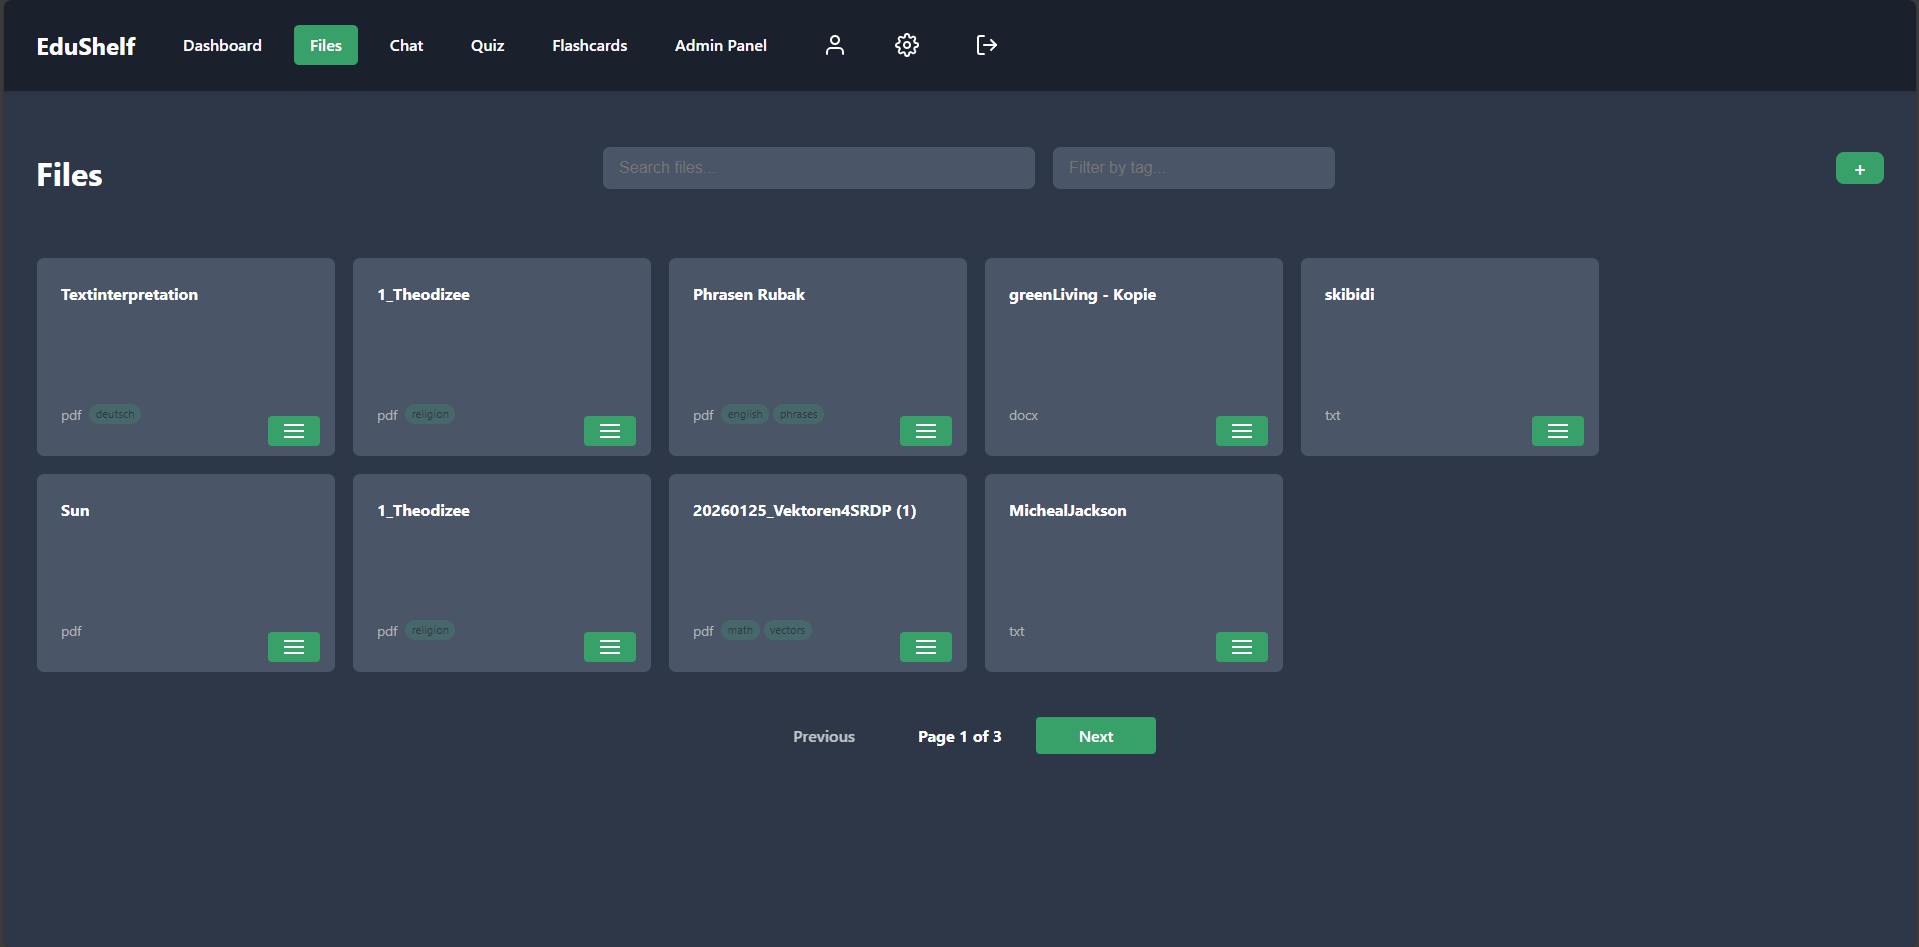
\includegraphics[width=0.92\textwidth]{img/files-dark-mode}
    \caption{Dateiansicht von EduShelf (Dark-Mode)}
    \label{fig:files}
\end{figure}

\subsection{Share-Dialog (ShareFileModal.jsx)}

Der Share-Dialog ist als kontrolliertes Formular implementiert. Der Nutzer gibt die E-Mail-Adresse oder den Benutzernamen der Zielperson ein. Da beide Eingabeformate akzeptiert werden, entfällt die Notwendigkeit, die genaue Identifikation des Empfängers zu kennen -- das Backend löst die Zuordnung auf.

\begin{lstlisting}[language=JavaScript, caption={Formularlogik im ShareFileModal}]
const ShareFileModal = ({ isOpen, onClose, onShare, fileName }) => {
    const [emailOrUsername, setEmailOrUsername] = useState('');
    const [isLoading, setIsLoading] = useState(false);

    const handleSubmit = async (e) => {
        e.preventDefault();
        if (!emailOrUsername.trim()) return;

        setIsLoading(true);
        try {
            await onShare(emailOrUsername); // Callback an Files.jsx
            setEmailOrUsername('');         // Eingabe nach Erfolg zuruecksetzen
        } finally {
            setIsLoading(false);
        }
    };
};
\end{lstlisting}

Während des Sendevorgangs wird der Submit-Button deaktiviert (\texttt{disabled={isLoading}}) und der Beschriftungstext wechselt von \textit{Share File} zu \textit{Sharing...}. Dieses Muster verhindert Mehrfach-Submissions und gibt dem Nutzer klares visuelles Feedback über den laufenden Prozess.

\subsection{Zustandsverwaltung für Shared Files}

Empfangene Freigaben erscheinen im Dateibereich des Empfängers mit einem visuellen Kennzeichen (\texttt{isShared: true}). Der Nutzer hat die Möglichkeit, eine Freigabe zu akzeptieren oder abzulehnen. Diese Entscheidung wird clientseitig im \texttt{localStorage} persistiert, da sie ausschließlich die Sichtbarkeit in der UI steuert:

\begin{lstlisting}[language=JavaScript, caption={Persistierung der Share-Entscheidungen im localStorage}]
// Akzeptieren einer Freigabe
const handleAcceptShare = (docId) => {
    const accepted = JSON.parse(
        localStorage.getItem('edushelf_accepted_shares') || '[]'
    );
    localStorage.setItem(
        'edushelf_accepted_shares',
        JSON.stringify([...accepted, docId])
    );
    fetchFiles(); // Listenaktualisierung ausloesen
};

// Ablehnen einer Freigabe
const handleRejectShare = (docId) => {
    const rejected = JSON.parse(
        localStorage.getItem('edushelf_rejected_shares') || '[]'
    );
    localStorage.setItem(
        'edushelf_rejected_shares',
        JSON.stringify([...rejected, docId])
    );
    fetchFiles();
};
\end{lstlisting}

\subsection{Bewertung des Ansatzes}

Die Entscheidung, den Accept/Reject-Status clientseitig zu speichern, hat sowohl Vor- als auch Nachteile. Der wesentliche Vorteil ist die sofortige Reaktivität ohne serverseitigen Roundtrip. Der Nachteil besteht in der fehlenden Geräteübergreifenden Synchronisation: Akzeptiert ein Nutzer eine Datei auf einem Gerät, ist sie auf einem anderen Gerät weiterhin als ausstehend markiert. Für eine zukünftige Version wäre eine serverseitige Persistierung des Share-Status daher erstrebenswert.
